\section {Résultats obtenus}

Tous les tests ont été réalisés sur la machine hôte \texttt{worf} de
la salle 203 décrite ci-après~:
\begin{itemize}
\item NVIDIA GF100GL Quadro 4000
\item Intel Xeon E7 v2/Xeon E5 v2/Core i7
\item Deux noeuds NUMA~:
  \begin{itemize}
  \item cache L3 15 MB
  \item 6 coeurs physiques avec hyperthreading~:
    \begin{itemize}
    \item cache L2 256 KB
    \item L1d 32 KB
    \item L1i 32 KB
    \end{itemize}
  \end{itemize}
\end{itemize}
On pourra retrouver la sortie de la commande \texttt{lstopo} en
annexes (figure~\ref{fig:lstopo}). Nous exécutons chaque méthode 5
fois puis nous faisons une moyenne des 5 mesures de temps.

\subsection{Comparaison des algorithmes séquentiels}

\begin{figure}[!ht]
  \center{
    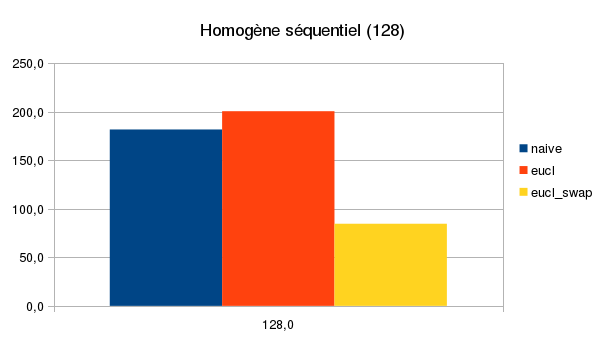
\includegraphics[width=10cm]{images/homoseq128.png}
  }
  \caption{}
  \label{fig:homoseq128}
\end{figure}

\begin{figure}[!ht]
  \center{
    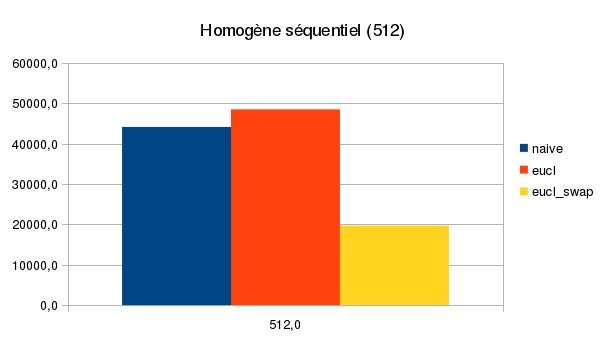
\includegraphics[width=10cm]{images/homoseq512.png}
  }
  \caption{}
  \label{fig:homoseq512}
\end{figure}

\begin{figure}[!ht]
  \center{
    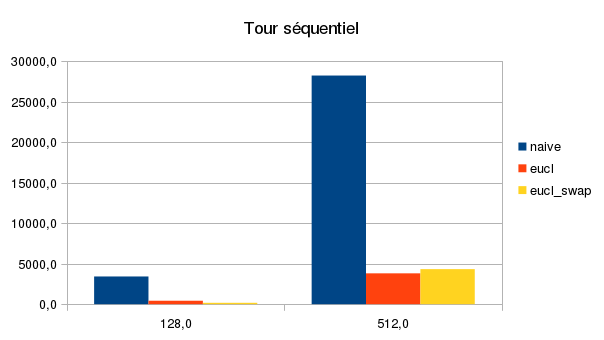
\includegraphics[width=10cm]{images/tourseq.png}
  }
  \caption{}
  \label{fig:tourseq}
\end{figure}

\subsubsection{Calcul naïf \textit{versus} division euclidienne}

La version qui utilise des divisions euclidiennes
\texttt{compute\_eucl} est 1,1 fois plus lente
(figure~\ref{fig:homoseq128} et~\ref{fig:homoseq512}) que la version
naïve \texttt{compute\_naive} pour les configurations homogènes. Cela
parait normal car les valeurs dans les cases à l'initialisation ne
dépassent pas 5. Ici, l'utilité de faire une division euclidienne est
limité.
\medskip

En revanche, pour le cas où on place un tas de 100000 grains au
centre, la version avec division euclidienne est 7 à 8 fois plus
rapide car on réduit le nombre d'itération nécessaire pour arriver à
stabilisation (figure~\ref{fig:tourseq}).

\subsubsection{Suppression des mauvaises prédictions de branchement}
\label{sec:predict}

La suppression de la condition qui vérifie si la valeur d'une case est
supérieure à la taille maximale d'un tas de sable améliore les
performances d'un facteur 3 environ pour la fonction
\texttt{compute\_eucl\_swap}.
\medskip

Grâce à l'optimisation de la section~\ref{sec:predict}, notre solution
\texttt{compute\_omp\_swap} qui limite les accès en écriture sur les
cases voisines est jusqu'à 2,5 fois plus rapide que les autres
méthodes séquentielles pour le cas homogène
(figure~\ref{fig:homoseq128} et~\ref{fig:homoseq512}). Sans la
suppression de la boucle, cette méthode est plus lente que les autres.

\subsubsection{chunk vector}

\subsection{Algorithmes multi-threads}

Sur les figures~\ref{fig:homopar128}, \ref{fig:homopar512},
\ref{fig:tourpar128}, et \ref{fig:tourpar512} on peut voir que la
méthode \texttt{compute\_omp} est plus lente que la méthode
\texttt{compute\_omp\_swap}. Cela peut s'expliquer par le surplus de
temps s'engendre l'étape de rapatriement des données dans la matrice
partagée, nécessaire après chaque itération.
\medskip

Les pics de speed-up correspondent aux exécutions avec un nombres de
threads multiples du nombres de lignes à traiter ($DIM-2$). Nous
pouvons voir l'intérêt de décourer la matrice en morceaux égaux entre
tous les threads.
\medskip

Sur les figures~\ref{fig:homopar512} et~\ref{fig:tourpar512} blabla

\begin{figure}[!ht]
  \center{
    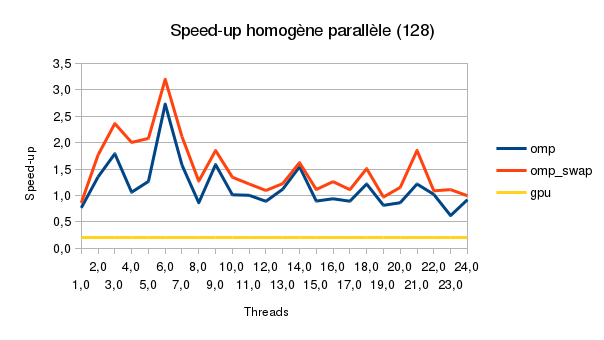
\includegraphics[width=10cm]{images/homopar128.png}
  }
  \caption{}
  \label{fig:homopar128}
\end{figure}

\begin{figure}[!ht]
  \center{
    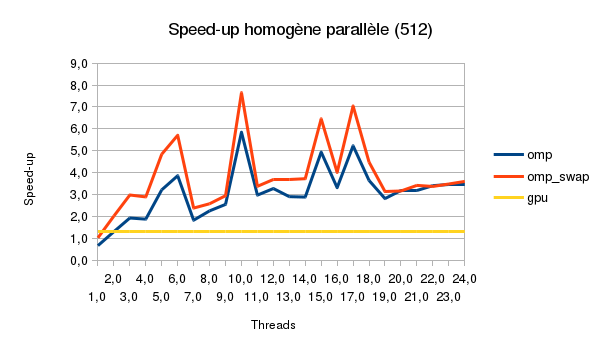
\includegraphics[width=10cm]{images/homopar512.png}
  }
  \caption{}
  \label{fig:homopar512}
\end{figure}

\begin{figure}[!ht]
  \center{
    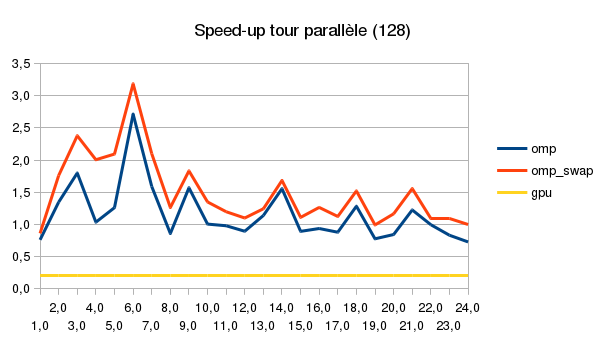
\includegraphics[width=10cm]{images/tourpar128.png}
  }
  \caption{}
  \label{fig:tourpar128}
\end{figure}

\begin{figure}[!ht]
  \center{
    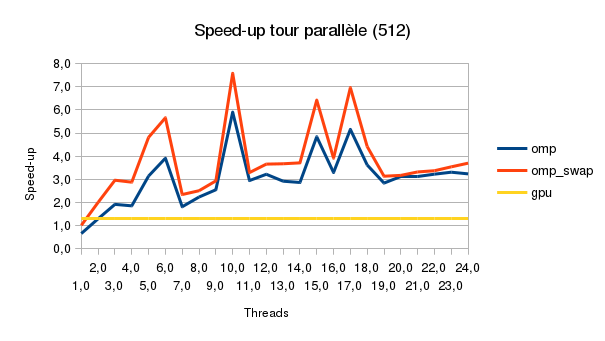
\includegraphics[width=10cm]{images/tourpar512.png}
  }
  \caption{}
  \label{fig:tourpar128}
\end{figure}
